\documentclass[aspectratio=169, hyperref={bookmarks=false}]{beamer}
\usepackage[T2A,T1]{fontenc}
\usepackage[english, russian]{babel}
\usepackage[utf8]{inputenc}

\hypersetup{unicode=true}

\usepackage{graphicx}
\graphicspath{{Plots/PDF/}}

\usepackage[export]{adjustbox}

\setbeamertemplate{navigation symbols}{}

\title{Поверхностная фотометрия галактик}
\subtitle{Отчет по галактике UGC 1198}
\author{Павел Соболев, Александр Крыжановский}
\date{}

\begin{document}

\frame{\titlepage}

\begin{frame}
\frametitle{Обработанное изображение галактики, фильтр B}

    \begin{minipage}[h]{\linewidth} 
    \center{\fbox{\includegraphics[trim={0 8cm 0 0}, max height=7cm,max width=7cm]{ObjectC}}}
    \end{minipage}

\end{frame}

\begin{frame}
\frametitle{Изофоты, фильтр B}

    \begin{minipage}[h]{0.9\linewidth} 
    \center{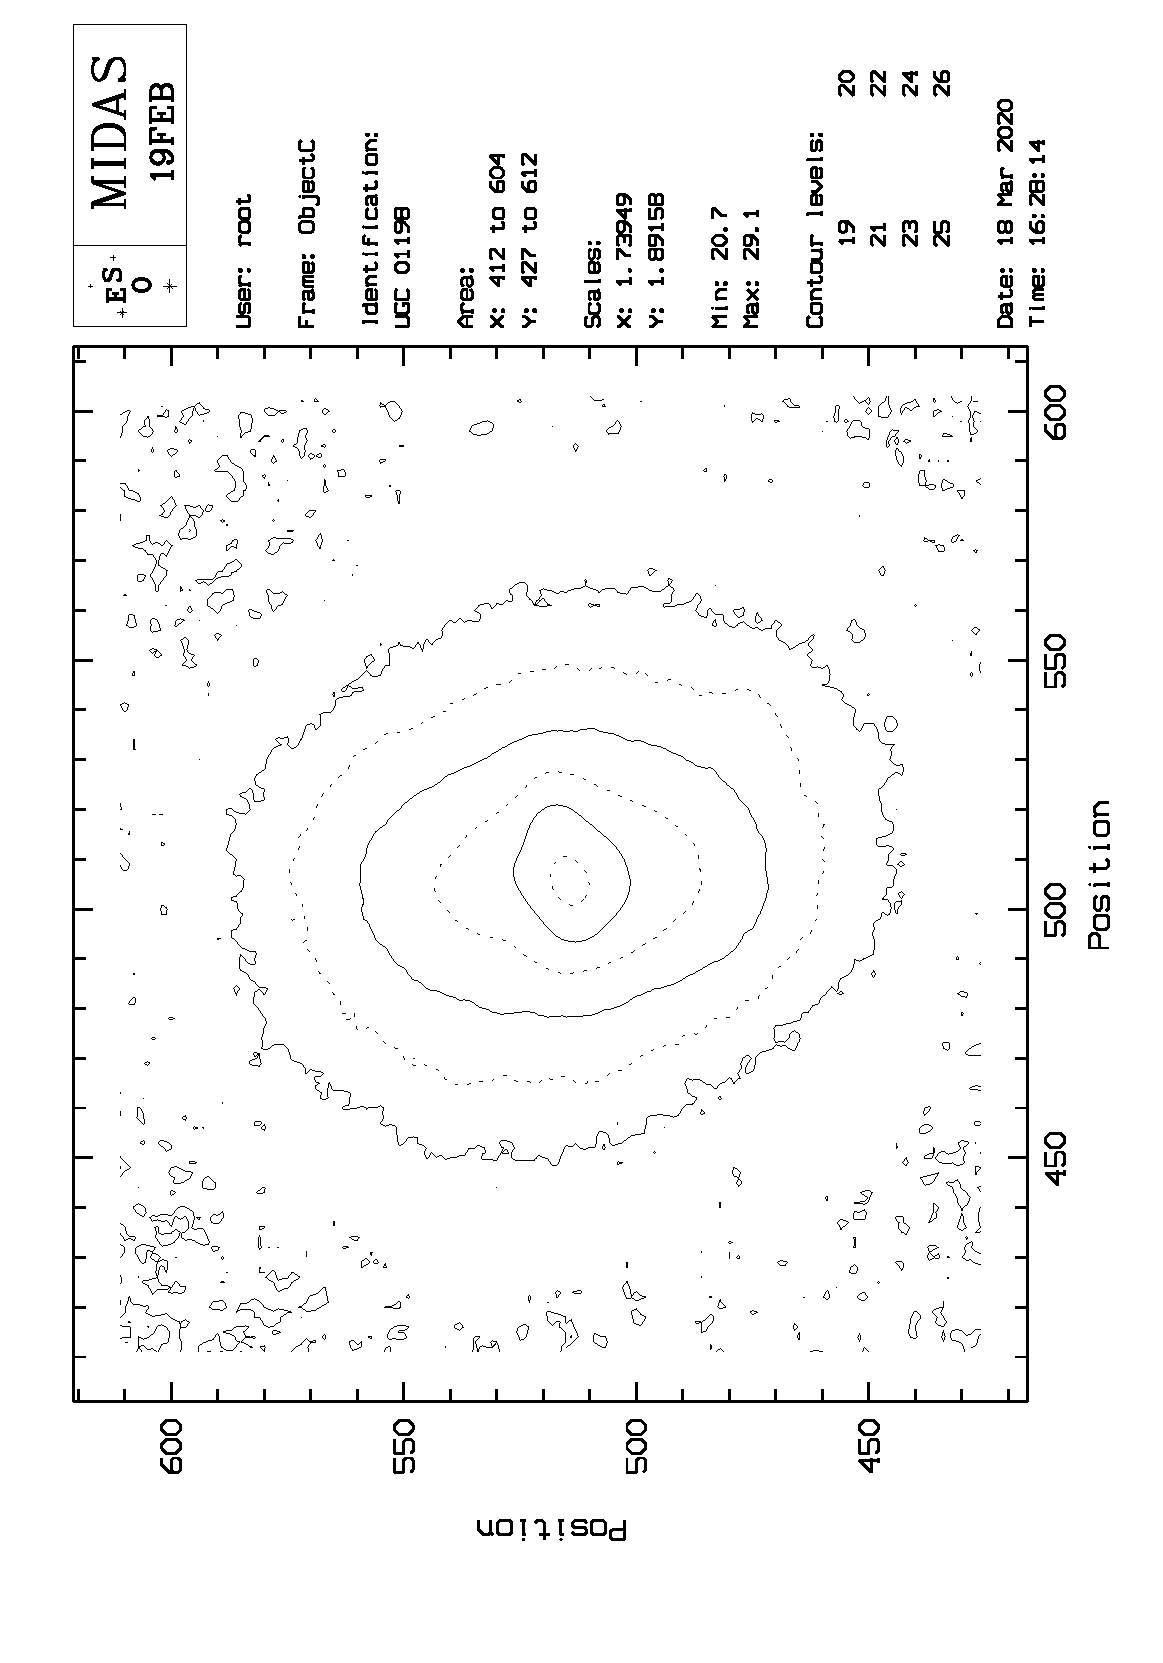
\includegraphics[totalheight=8cm]{Isophote}}
    \end{minipage}

\end{frame}

\begin{frame}
\frametitle{Разрезы, фильтр B}

    \begin{minipage}[h]{0.9\linewidth}
    \center{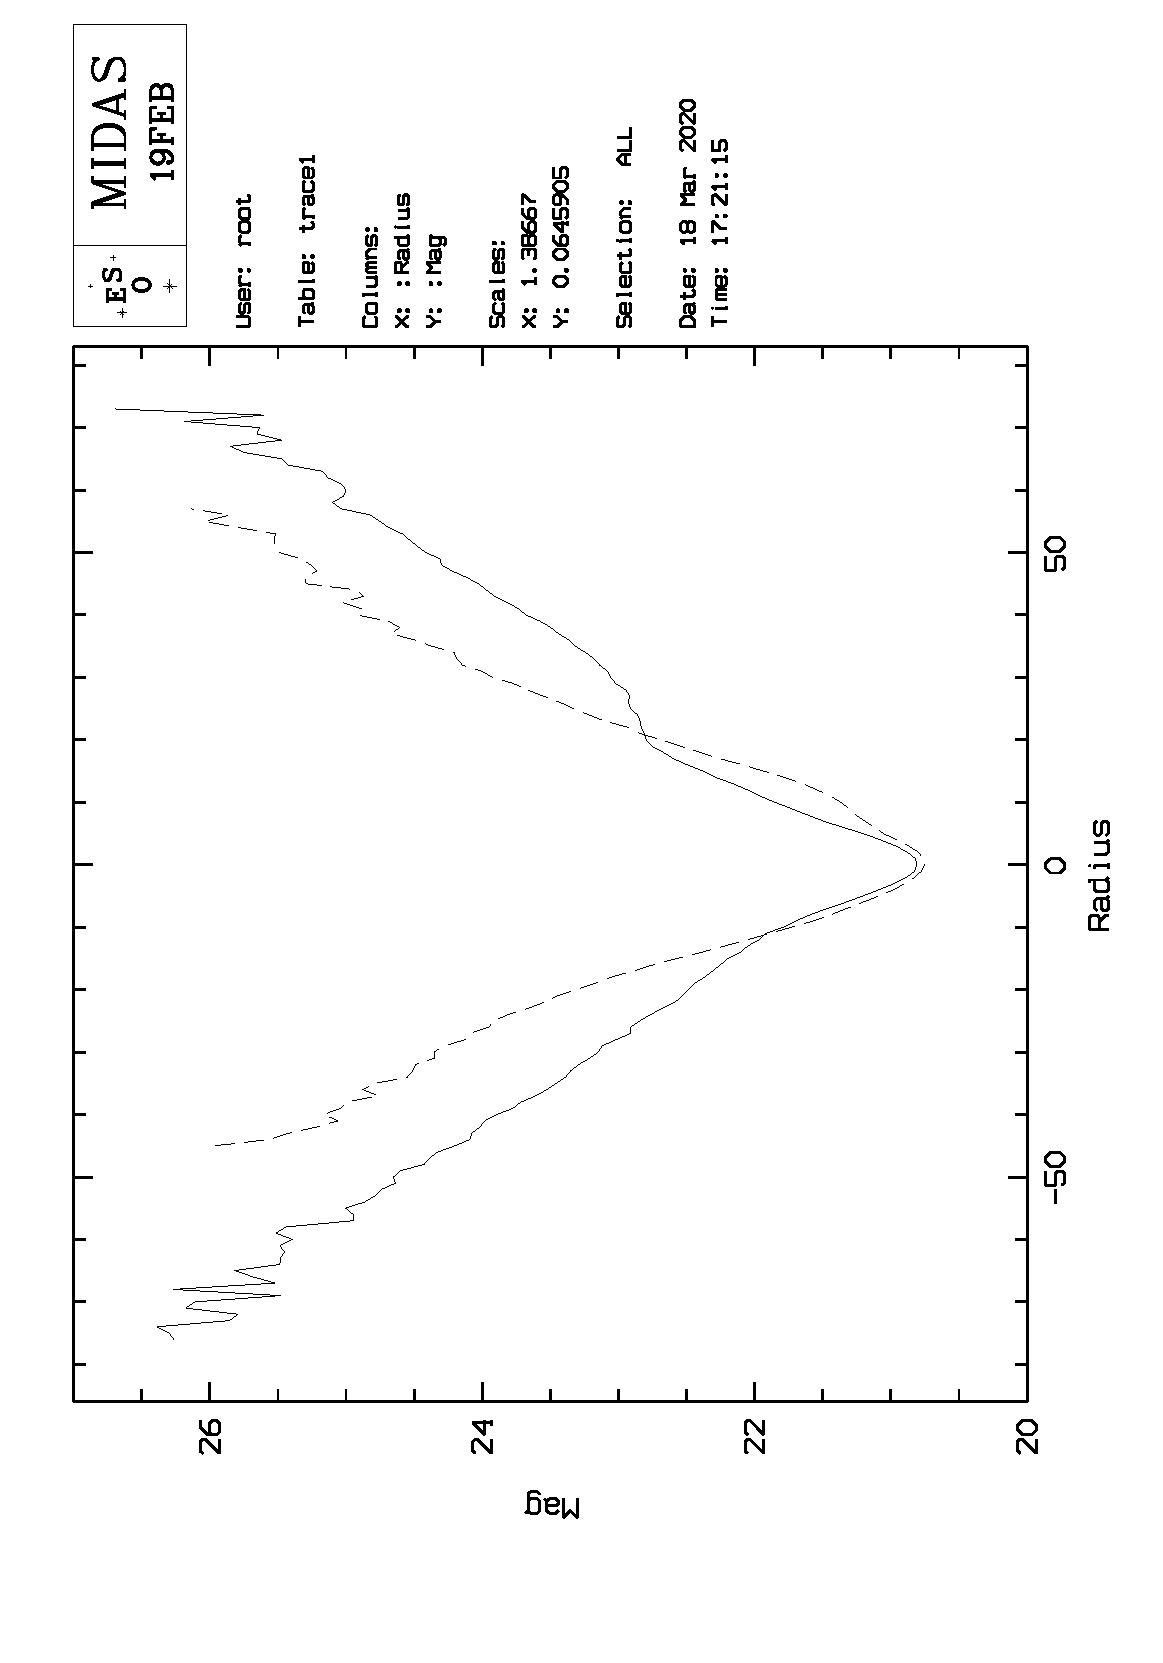
\includegraphics[totalheight=8cm]{Cuts}}
    \end{minipage}

\end{frame}
 
\end{document}
